% -----------------------------------------------
% Template for ISMIR Papers
% 2020 version, based on previous ISMIR templates

% Requirements :
% * 6+n page length maximum
% * 4MB maximum file size
% * Copyright note must appear in the bottom left corner of first page
% * Clearer statement about citing own work in anonymized submission
% (see conference website for additional details)
% -----------------------------------------------

\documentclass{article}
\usepackage[T1]{fontenc} % add special characters (e.g., umlaute)
\usepackage[utf8]{inputenc} % set utf-8 as default input encoding
\usepackage{ismir,amsmath,cite,url}
\usepackage{graphicx}
\usepackage{color}
\usepackage[]{algorithm2e}

% Optional: To use hyperref, uncomment the following.
% \usepackage[bookmarks=false,hidelinks]{hyperref}
% Mind the bookmarks=false option; bookmarks are incompatible with ismir.sty.

\usepackage{lineno}
\linenumbers

% Title.
% ------
\title{Improving Fairness in Music Recommendation Prediction}

% Note: Please do NOT use \thanks or a \footnote in any of the author markup

% Single address
% To use with only one author or several with the same address
% ---------------
%\oneauthor
% {Names should be omitted for double-blind reviewing}
% {Affiliations should be omitted for double-blind reviewing}

% Two addresses
% --------------
%\twoauthors
%  {First author} {School \\ Department}
%  {Second author} {Company \\ Address}

%% To make customize author list in Creative Common license, uncomment and customize the next line
%  \def\authorname{First Author, Second Author}


% Three addresses
% --------------
\threeauthors
  {First Author} {Affiliation1 \\ {\tt author1@ismir.edu}}
  {Second Author} {\bf Retain these fake authors in\\\bf submission to preserve the formatting}
  {Third Author} {Affiliation3 \\ {\tt author3@ismir.edu}}

%% To make customize author list in Creative Common license, uncomment and customize the next line
%  \def\authorname{First Author, Second Author, Third Author}

% Four or more addresses
% OR alternative format for large number of co-authors
% ------------
%\multauthor
%{First author$^1$ \hspace{1cm} Second author$^1$ \hspace{1cm} Third author$^2$} { \bfseries{Fourth author$^3$ \hspace{1cm} Fifth author$^2$ \hspace{1cm} Sixth author$^1$}\\
%  $^1$ Department of Computer Science, University , Country\\
%$^2$ International Laboratories, City, Country\\
%$^3$  Company, Address\\
%{\tt\small CorrespondenceAuthor@ismir.edu, PossibleOtherAuthor@ismir.edu}
%}
%\def\authorname{First author, Second author, Third author, Fourth author, Fifth author, Sixth author}


\sloppy % please retain sloppy command for improved formatting

\begin{document}

%
\maketitle
%
\begin{abstract}


Recommender systems are an important tool used by music streaming
platforms. These systems facilitate the recommendation of new songs
and artists to their users. Increasingly, music recommendations 
are influencing user listening behavior,
which naturally impacts the music
industry, as well as cultural and social aspects of our society. 
This has opened up a research area, namely the identification 
of biases introduced by recommender systems in the music context.

Recent research, which focused on users of 
the Last.fm platform, found that state-of-the-art music recommendation 
systems frequently tend to give favor to already popular items.
To this end, we propose a new method for predicting
music recommendations. By assuming the distribution of
the popularity of artists to be a Gaussian Mixture,
we estimate three different popularity clusters, 
and make the predictions of the recommendation
algorithms in a way that it respects the cluster 
distribution.
Our final predictions are able to increase
the recommendation frequencies of less popular artists, while 
preserving the specific characteristics of each algorithm.
The GAP(g)$_r$ and 
Mean Average Error (MAE)
metrics are improved, showing that our recommendations 
are more accurate and approximate to the expected 
popularity of the artists in each user profile. 

%For such reasons, researchers have recently been
%turning their attentions to investigating 
%the possible biases introduced by recommender systems in 
%the music context. 


\end{abstract}
%
\section{Introduction}\label{sec:introduction}


Recommender systems are an important tool used by music streaming
platforms in general. These systems facilitate the recommendation
of new songs and artists to their users, and have become more
common in recent years. Nowadays the current
widespread use of streaming platforms makes music
recommendations play an increasingly important role in
users' listening behavior and their curiosity towards new 
musical experiences. For such reasons, 
recommendation algorithms naturally impact the music
industry,
as well as cultural and social aspects of our society \cite{music_taste}. 

This has opened up an area of research, namely the identification 
of biases introduced by recommender systems in the music context.
Recently, an investigation of the aspects of music recommendation diversity led to a discussion of the importance of being concerned with diversity in MIR \cite{recommendationdiversity}.
In a similar
way, capturing and being in accordance with the cultural 
background of listeners has been listed as one
of the current major challenges for 
recommendation algorithms \cite{challenge}. 

Artist popularity, by its turn, is a major component 
when discussing fairness for music recommendations.
It is no news that recommendation algorithms
tend to favor the most popular artists
\cite{celma2008hits, pap_unfairness}, leading
the less-known ones to be under-represented in the predictions. This not
only directly affects less popular artists, but it also
puts the algorithms at the risk of not actually
recommending novel music to the users. Reasonably, if a user
gets recommended popular artists that are similar
to what they already listen to, it is likely that
these recommendations will not be novel \cite{celma2008hits}.

Furthermore, in \cite{pap_unfairness} the researchers not
only investigate the popularity bias patterns in 
music recommendation algorithms, but also raise questions about
how to improve the current situation. In light of that, 
the focus of this paper is to propose an adaption
to the way predictions are made for recommender systems. The emphasis of the proposed method is in reducing the
popularity bias in the predictions. This is accomplished
by assuming the distribution of the popularity of artists
has have a latent grouping variable, and afterward by
predicting the recommendations in a way that
respects this cluster distribution. The adapted predictions
are made stochastically, by means of introducing 
a sampling stage in the prediction process. Besides, by 
changing the prediction methodology rather than the algorithms
themselves, we allow the proposed technique to be widely applicable
to algorithms not contemplated in the experiments of
the present work. 

This document is structured as follows. 
Section 2 provides an overview on
fairness for Music Recommender Systems. 
After that, we propose and explain a new methodology for improving fairness in music recommendation prediction. Results are presented in 
Section 4, which is followed by the conclusions 
in Section 5. 




%Introduction: what is music recommendation, what is it important 
%for, why does it need to be fair; 1 page


%stochastic, general method
% mention the main reference and how this is based on
% that






\section{Fairness in Music Recommendation}\label{sec:unfairness}


We now briefly discuss what fairness means
in the context of music recommendations. 
Though there is no closed definition that 
comprises all elements involved in the fairness
of an algorithm, we will focus on the elements that are 
relevant to the context of this paper. 

Fairness in recommendations can consider whether
an algorithm behaves equally across different user 
groups \cite{ekstrand2018all}. In other words, if a 
system is not effectively replicating the taste of specific 
groups, while others have their preferences well 
captured, it can be considered unfair. This 
grouping can have various definitions 
(demographic, usage behavior, age, etc). 
As for music recommender systems, recent research 
has demonstrated that the algorithms can 
discriminate by mainstreaminess user level \cite{van2013deep}.
This makes mainstreaminess, a metric that reflects user
inclination to mainstream music, one characteristic of 
interest in the music recommendation fairness 
scenario \cite{pap_unfairness}. 

On the other hand, fairness can also be defined 
from the point of view of the artists. 
If we take into consideration the equitable treatment of 
content producers, when some artists are significantly 
recommended more times than others, the algorithm used 
might be considered unfair as well. In this sense, 
the popularity bias is a source of concern, as it has
been observed that popular artists tend to get recommended
more often by state-of-the-art recommendation algorithms
\cite{celma2008hits, pap_unfairness}. 

For this work, we are interested in the
two characterizations: fairness from the
perspective of the users and from
the perspective of the artists. We will 
later show how our method is able to give a more
fair treatment to the artists, while still
keeping a good algorithm accuracy for three
different user groups, which is related to the
fairness to the users' preferences. 


\section{Adapting Predictions}\label{sec:methods}

%\subsection{Adapting Recommendation Prediction}\label{sec:adapt}

Music recommender systems are algorithms capable of giving
artists a rating that measures how likely each user is to 
enjoy their songs. The traditional method then recommends the
$\mathbf{n}$ artists with the highest predicted ratings for the user.
By the way the algorithms are constructed, this manner
of making predictions is natural, and usually is not the
object of study when recommendation fairness is discussed. 

The following proposed method aims to reduce the popularity
bias in predictions by introducing a latent grouping variable into the distribution of the popularity of artists. The predictions are then made in a way that
respects this cluster distribution.
These adapted predictions
are made stochastically, by introducing
a sampling stage in the prediction process. 

First, let us define a set of users $\mathcal{U}$, 
their music consumption history $\mathcal{I}_{\mathcal{U}}$,
the set of artists $A_{\mathcal{I}}$ in their history, and
the popularity of these artists as $\boldsymbol{Pop}_{A}$. 
Our goal here is to describe a method for making
predictions $\boldsymbol{p}$ using a recommender system
such that artists with high popularity are not favored
at the expense of ones with low popularity. 

We start by assuming the existence of a
hidden variable $z_k, k  \in \{1,\dots,K\}$ 
in the artist popularity distribution and estimate
its parameters. This clustering variable shall 
characterize the different popularity groups present in 
the data. We do not limit the techniques that 
can be employed in the estimation of the latent
variable, but for this work we make
use of a Gaussian Mixture model
\cite{murphy2012machine}. 

We do that by assuming the popularity variable for a given
artist $i$, 
$\boldsymbol{Pop}_{A}_{i}$, to be distributed as a 
Gaussian Mixture, which can be formulated as

$$ \mathcal{P}(\boldsymbol{Pop}_{A}_{i} |\boldsymbol{\theta}) = 
\sum_{k = 1}^{K} \pi_k \mathcal{N}(\boldsymbol{Pop}_{A}_{i}   | \boldsymbol{\mu}_k, \boldsymbol{\Sigma}_k),$$

where $\pi_k, k \in \{1,\dots,K\}$ can be seen as
the estimated proportions of each  cluster
\cite{murphy2012machine}. The optimal number of clusters
is unknown but can easily be determined by analyzing 
the Bayesian Information Criterion (BIC) for a set of
different chosen $K$ values.

After the Gaussian Mixture is fit, we adapt 
the recommendation predictions in a way that it
respects the estimated cluster distribution. First, 
we specify a value $m$ and use the estimated $\boldsymbol{\pi}$
as an approximation to the proportion 
parameters of a Multinomial distribution, and for each user in $\mathcal{U}$, sample 
an $(m_1,\dots, m_{K})$. The recommendation algorithm
of choice is fit, and its predicted ratings for each 
user is extracted. Then,  
instead of selecting the artists with the highest ratings
(classical top-$n$ methodology), 
we select the $(m_1,\dots, m_{K})$ artists
from clusters $(1, \dots, K)$ as the final recommendations. 
More details are given in Algorithm \ref{alg:method}. 



\RestyleAlgo{boxruled}
\begin{algorithm}[ht]
\label{alg:method}
 \KwData{Recommendation algorithm, $\mathcal{I}_{\mathcal{U}}$}
 \KwResult{Adapted predictions $\mathbf{p^{*}}$}
  \textbf{Initialisation\;}
  Fit a recommendation algorithm for $\mathcal{U}$ based on $\mathcal{I}_{\mathcal{U}}$; \\
  Set $(\pi_1,\dots, \pi_{K})$ to be approximately 
  the estimated proportions 
  for the popularity clusters $(z_1,\dots,z_k)$; \\
  Set \textbf{n} as the initial number of top predictions; \\
  Set $\textbf{m} \leq \textbf{n}$ as the final number of adapted predictions; \\
  Set \textbf{U} as the total number of users; \\
  Set \textbf{K} as total the number of estimated popularity clusters;
  
 \For{iteration i from 1 to U}{
  Get the top \textbf{n} rating predictions $\mathbf{p_i}$ for user $\mathbf{i}$;\\
  Predict the popularity clusters $\mathbf{z_{k}}$ for the artists in $\mathbf{p_i}$; \\
  
  Set $(m_1,\dots, m_{K})$ as a sample from a Mu$(\textbf{m}, \boldsymbol{\theta} \approx (\pi_1,\dots, \pi_{K}))$;\\ 
  
  Set $(m_1,\dots, m_{K})$ as the number of 
  artists from clusters $(z_1,\dots, z_{K})$ that will 
  be in the final predictions; 
  
  \For{iteration j from 1 to K}{
  Get the top $m_j$ artists that are in cluster $z_j$ from 
  $\mathbf{p_i}$ and add them to the final predictions $\mathbf{p^{*}_{_i}}$
  }
  Use $\mathbf{p^{*}_{_i}}$ as the final predictions for user $\mathbf{i}$;\\
 }
 \caption{Adapting Music Recommendation Prediction}
\end{algorithm}



By picking the artist predictions in this fashion, we 
allow the popularity distribution to be better represented, 
while still preserving the characteristics of each 
recommendation algorithm. The adapted predictions
are made stochastically with the introduction of 
the Multinomial sampling stage.
However, we
do not advise for the straightforward use of $\boldsymbol{\pi}$
as the proportion parameters of the Multinomial, given
that these estimated values might be too low for one or
more cluster labels. In a different
approach, one can also choose to optimize these parameters
depending on their specific goals. 



\section{Experiment Details}\label{sec:methods}

In this section, we describe the data and 
the recommendation algorithms used, as well as other details of our experiments. 

\subsection{Data}\label{sec:data}

For this work, we use the same data as \cite{pap_unfairness},
the widely used LFM-1b dataset \cite{lastfm}, 
composed by 1.1 billion listening events of 120,322 unique users
on the Last.fm\footnote{https://www.last.fm/} platform. For comparison consistency, 
we extract the same subsample of this data as
\cite{pap_unfairness}, ending up with a final dataset
of 3,000 users separated into three mainstreaminess groups:
low (1000 users), medium (1000 users) and high (1000 users)
mainstreaminess. The mainstreaminess metric used
is a proxy to the user's inclination toward popular
artists, and is defined  as the
overlap between the users listening history and 
the aggregated listening history of all Last.fm users
in the original dataset \cite{bauer2019global}. 
Recent research 
has demonstrated that the currently employed algorithms have the potential to 
discriminate by mainstreaminess user level \cite{van2013deep}.
Splitting the users be mainstreaminess
helps us observe the results of our method in 
groups of users with different behaviors. As for the train/test split, 
we use the traditional 80/20 rule. 



\subsection{Recommendation Algorithms}\label{sec:algorithms}


In \cite{pap_unfairness}, 6 different 
recommendation algorithms are evaluated:
(i) Random, (ii) Most Popular, (iii) 
User Item Average \cite{koren2010factor},
(iv) User KNN
\cite{schafer2007collaborative}, 
(v) User KNN Average (User KNN combined
with User Item Average), and (vi)
Non-Negative Matrix Factorization (NMF)
\cite{luo2014efficient}. In the present
work, we limit ourselves to investigating
the last 
four methods, considering 
that the Random and Most Popular
algorithms are in the popularity fairness
extremes: the first can be completely
fair to the artists 
but not well personalized to the users,
while the second will specifically favors
only the most popular artists \cite{pap_unfairness}.

Though, due to computational constraints, our experiments are only based on the four algorithms listed
above, we
acknowledge that recommendation systems is a rich 
research area, with novel algorithms being 
rapidly proposed.  Luckily, our method can
be widely applied and extended to other algorithms naturally, as
it does not add any algorithm dependent or computationally
expensive steps. 



\section{Results}\label{sec:methods}

This section presents the results in terms of the 
clusters estimated, and the fairness and accuracy of our
proposed method.


\subsection{Popularity Clustering}\label{sec:pop_cluster}


\begin{figure}[ht]
 \centerline{
 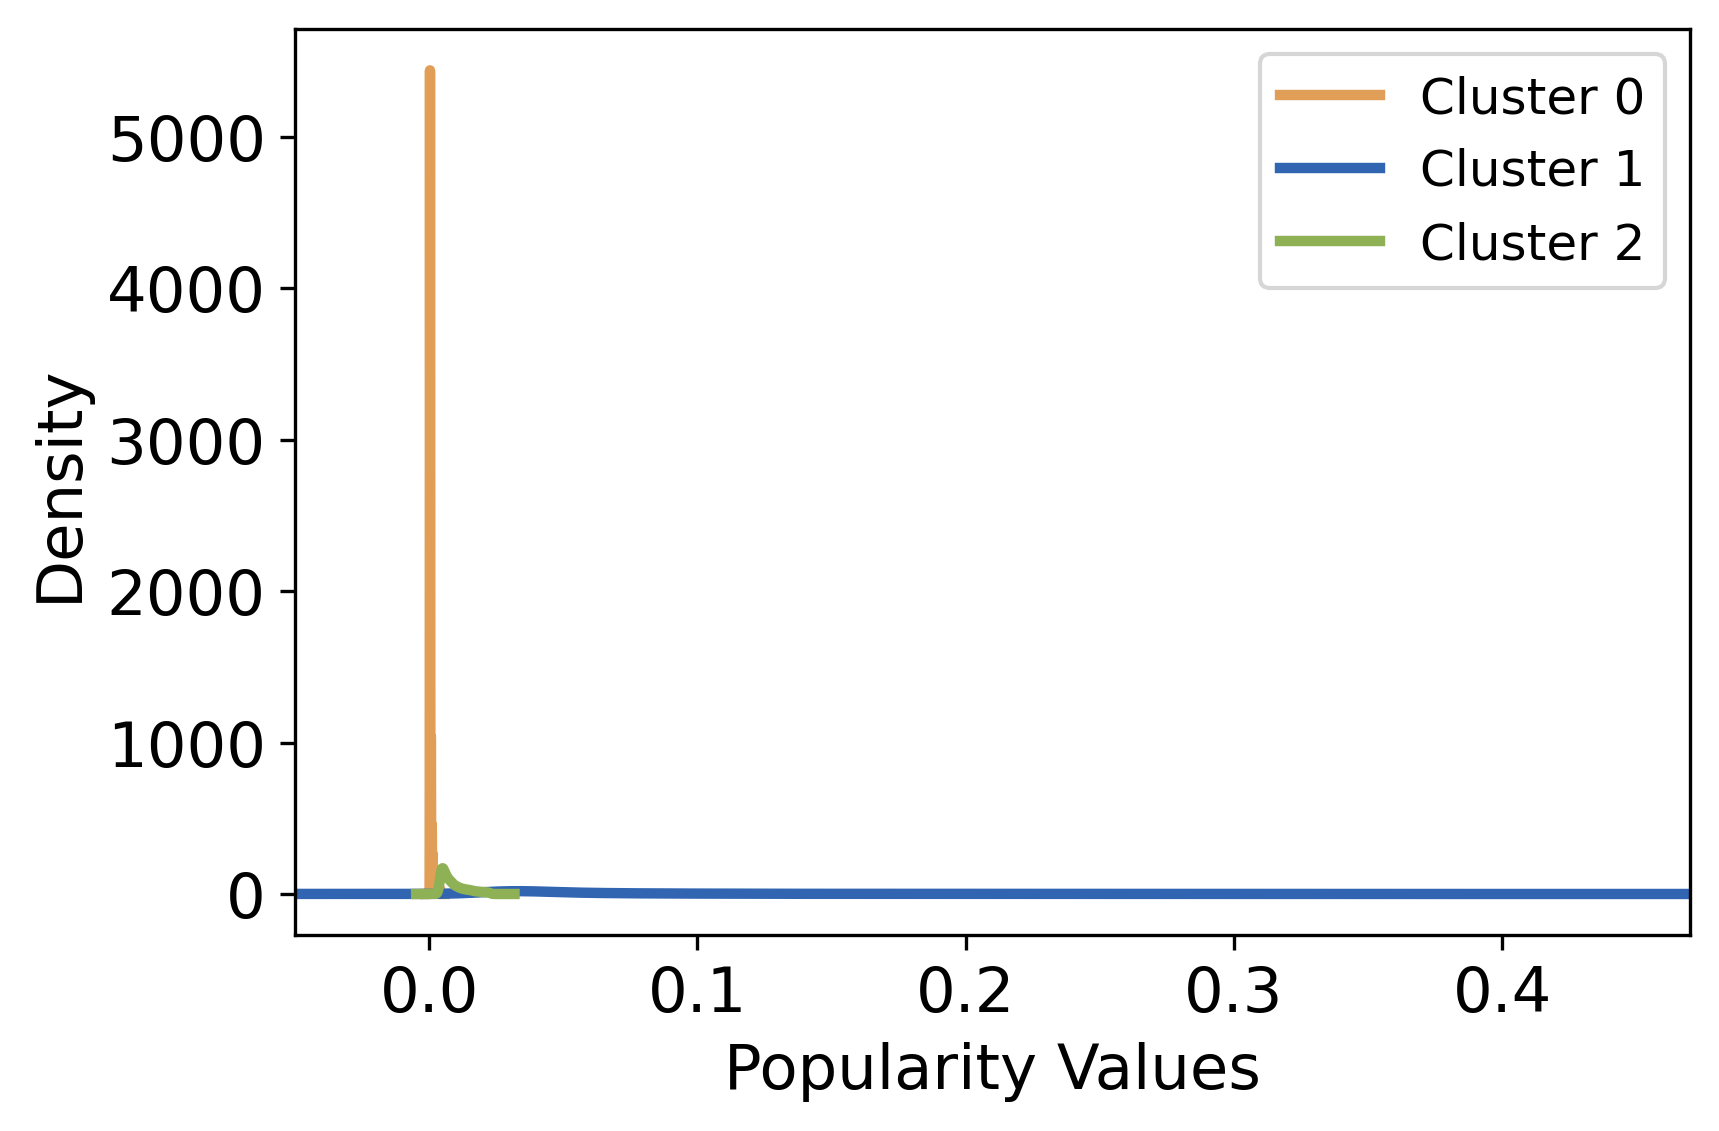
\includegraphics[width=\columnwidth]{img/clusters.png}}
 \caption{Densities for the estimated popularity clusters. Proportions are aproximately: 94.3\% for Cluster 0 (low popularity),  1\%  for Cluster 1 (high popularity), and 4.6\%  Cluster 2 (medium popularity). The maximum calculated value for popularity is 0.463.} 
 \label{fig:clusters}
\end{figure}

Unsurprisingly, the empirical density of the artists' popularity
is very skewed to the right (long tail), 
implying that most artists are of low to medium popularity
(Figure \ref{fig:clusters}). As the first step of our approach, we estimate the popularity clusters 
using a Gaussian Mixture Model. The values $K \in (2, \dots, 9)$ were tested
for the number of clusters, and the resulting 
$K = 3$ was selected with the help of the BIC. In Figure
\ref{fig:clusters}, we present the empirical 
densities of the resulting popularity clusters. If we have to label each
cluster, we could call them the low (Cluster 0), medium (Cluster 2)
and high (Cluster 1) popularity clusters, as implied by the plot. 
The mixing proportions are estimated to be 
$\pi_1 = 0.943$ (low popularity cluster), 
$\pi_2 = 0.01$ (high popularity cluster), 
and  $\pi_3 = 0.046$  (medium popularity cluster). The fitted
Gaussian Mixture model is then used to allocate each artist to a
cluster, which is later used as detailed in Algorithm \ref{alg:method}. 

Concerning the final proportion parameters of the 
Multinomial distribution, we used 
$(\theta_1, \theta_2, \theta_3) = (0.9, 0.03, 0.07)$.
Those values are based on $(\pi_1, \pi_2, \pi_3)$
but are not the same, given that the original
$\pi_1$ is very high, while 
$\pi_2$ is too low. As we do not want 
to reduce the popularity bias at the expense
of the model accuracy, using too low or too
high values could be harmful to the algorithm.


% mention that this is not what we used as cluster proportions

\subsection{Recommendation Fairness}\label{sec:pop_cluster}

%When we are concerned with the popularity bias of an algorithm, 
%%it is appropriate to investigate its behavior regarding 
%the popularity bias of the recommendations produced.



\begin{figure}[ht]
\centering
\begin{tabular}{cc}
  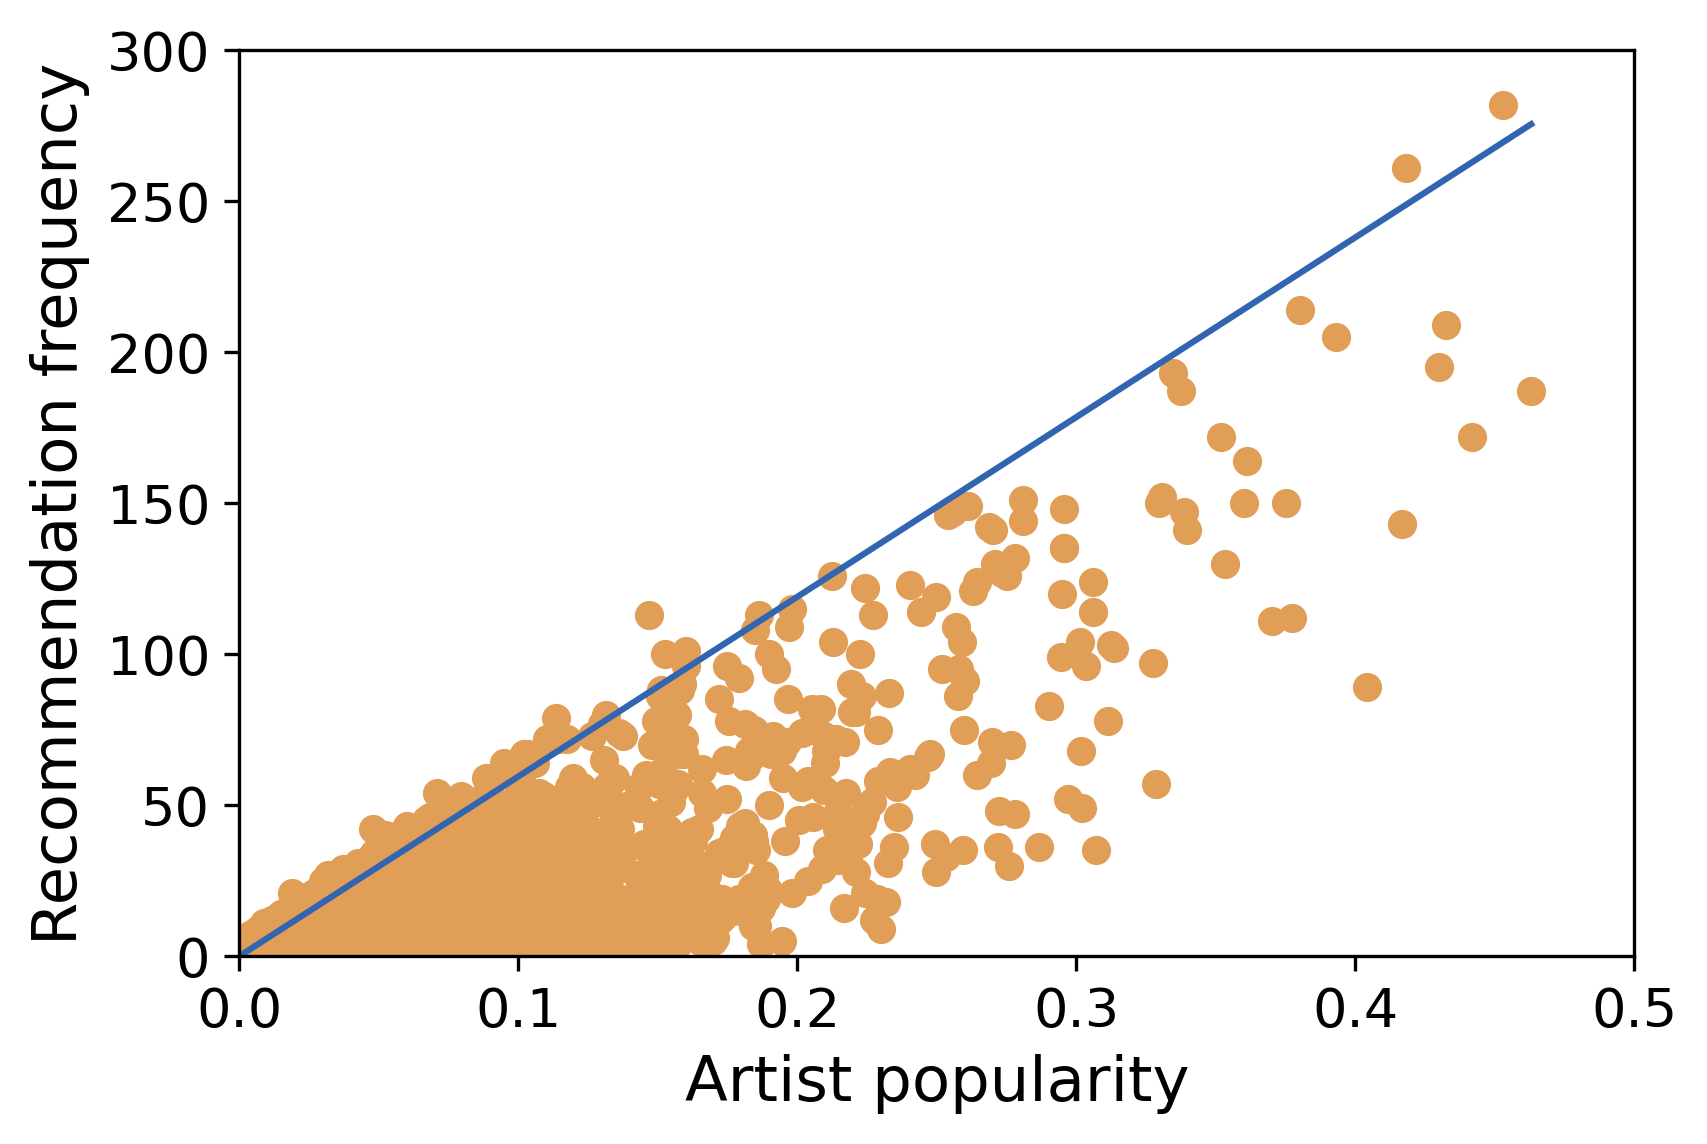
\includegraphics[width=35mm]{img/sampl_28_UserKNNAvg.png} &   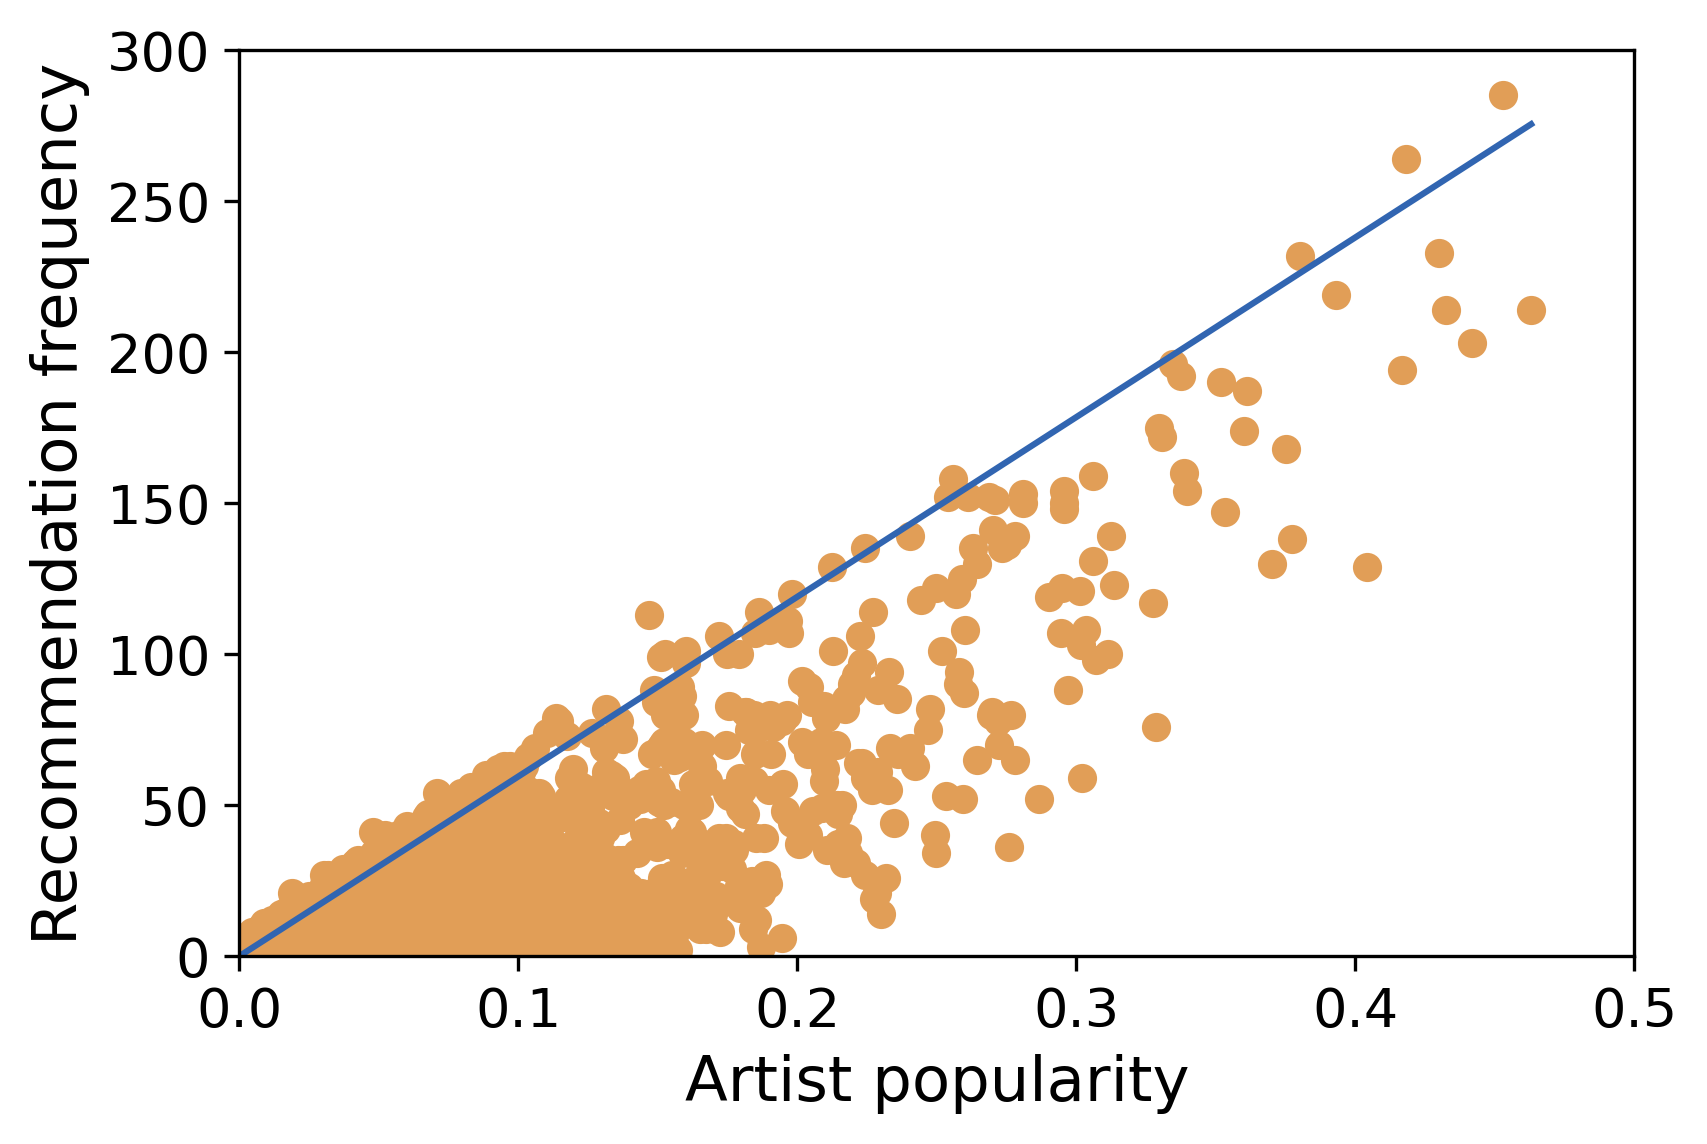
\includegraphics[width=35mm]{img/sampl_28_UserKNN.png} \\
(a) UserKNNAvg & (b) UserKNN \\[6pt]
 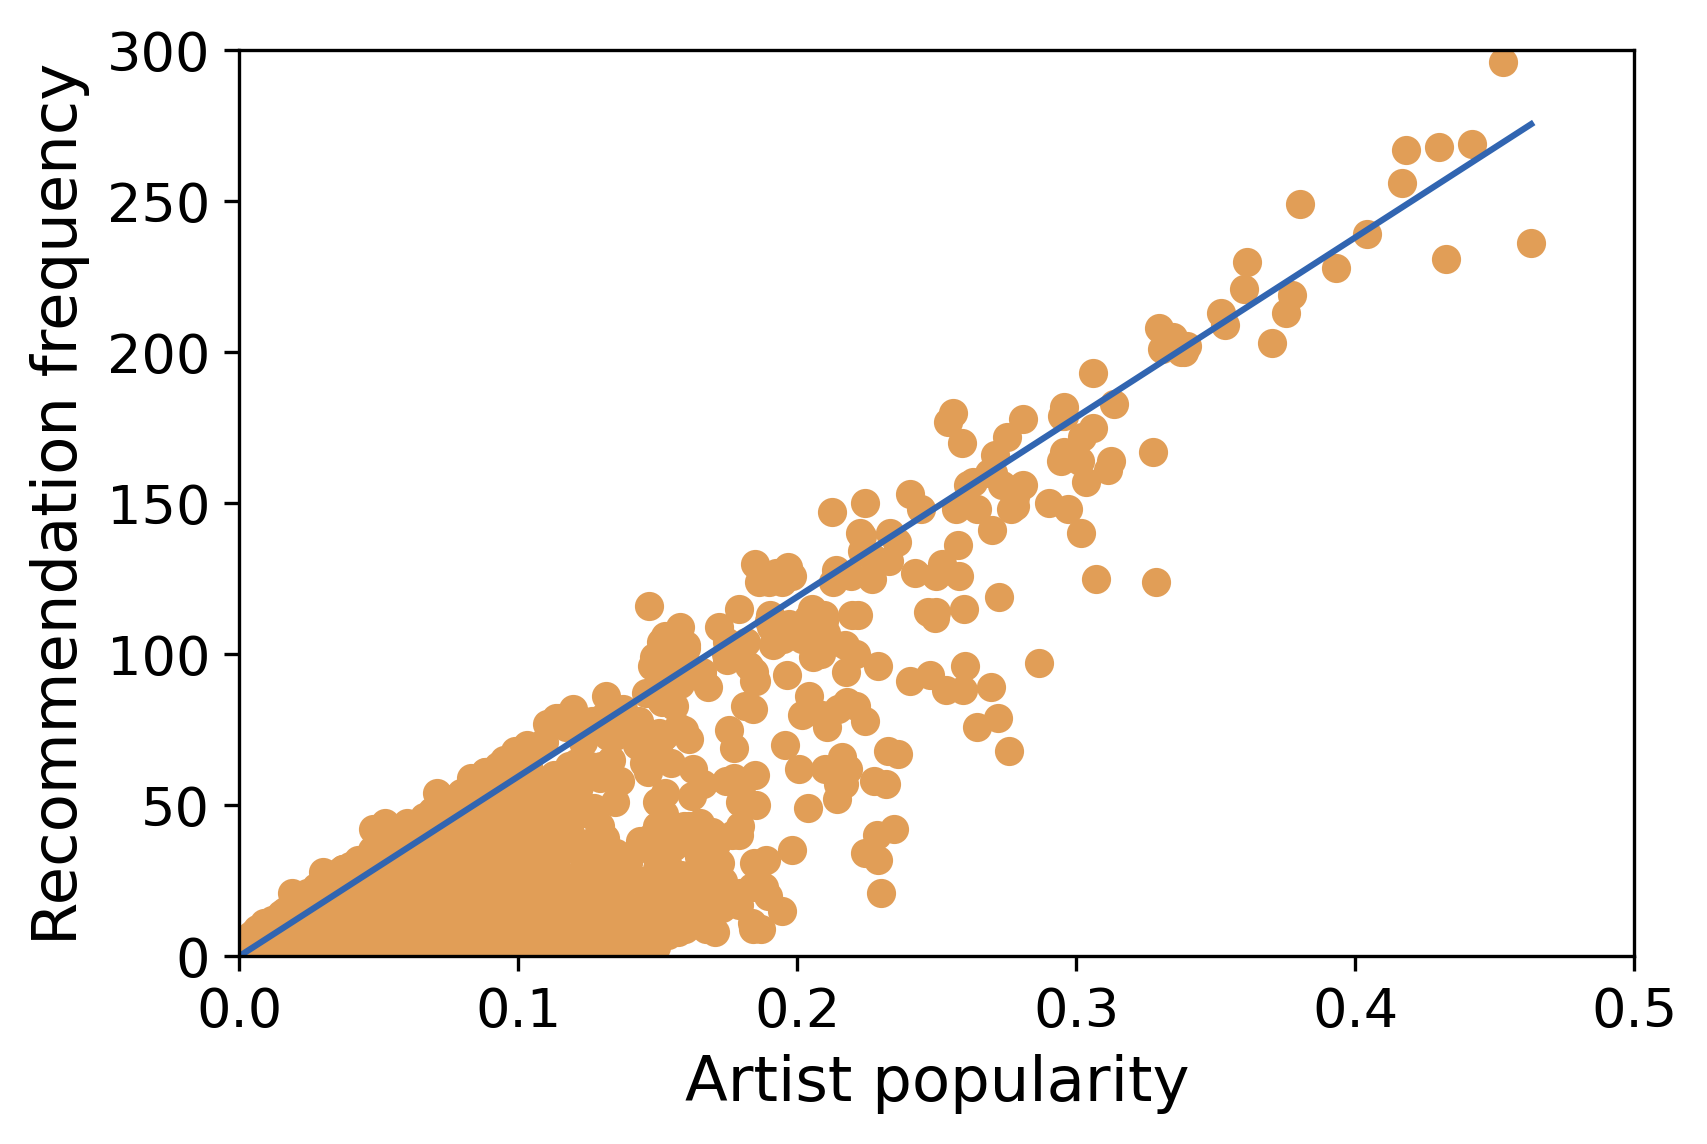
\includegraphics[width=35mm]{img/sampl_28_UserItemAvg.png} &   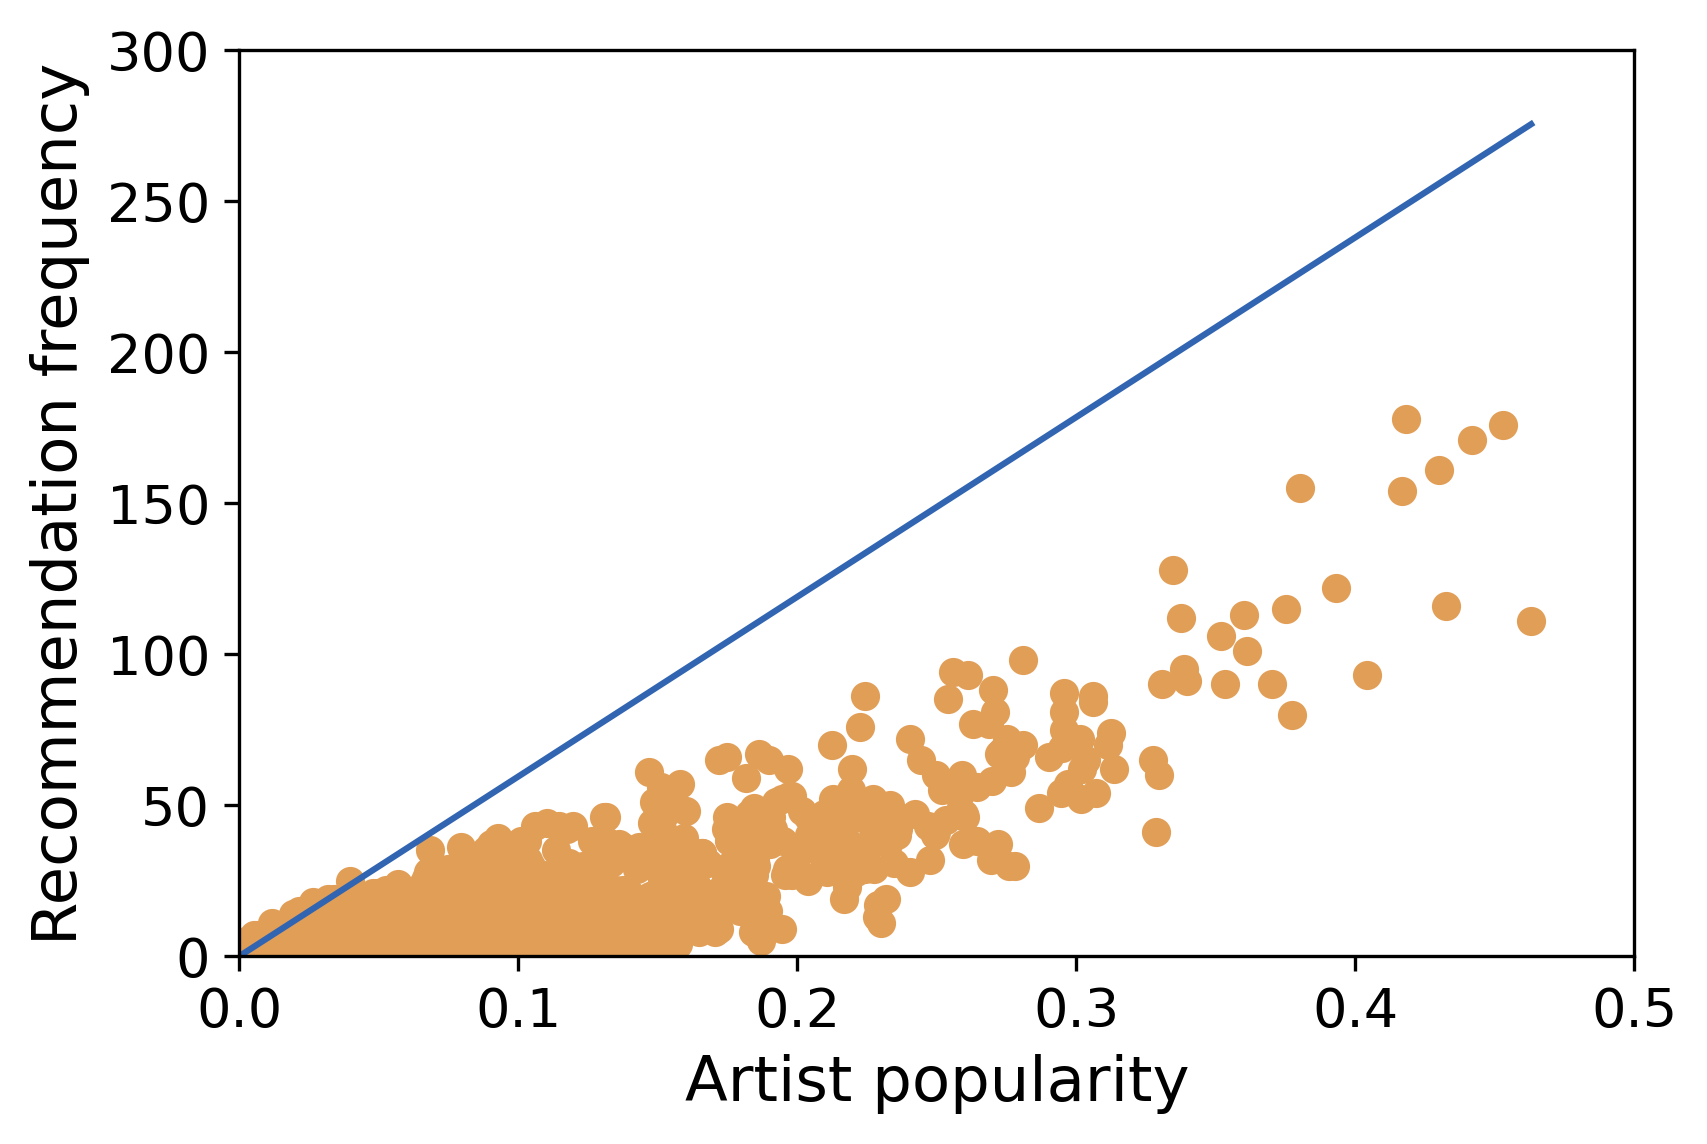
\includegraphics[width=35mm]{img/sampl_28_NMF.png} \\
(c) UserItemAvg & (d) NMF \\[6pt]
\end{tabular}
\caption{Artist popularity against recommendation frequencies, using the Top 28 artists as the predictions (standard method).
The blue straight line is for reference only and is positioned in the same coordinates for all plots. 
For all algorithms, the recommendation frequency increases 
with popularity.}
\label{fig:std}
\end{figure}


\begin{figure}[!ht]
\centering
\begin{tabular}{cccc}
  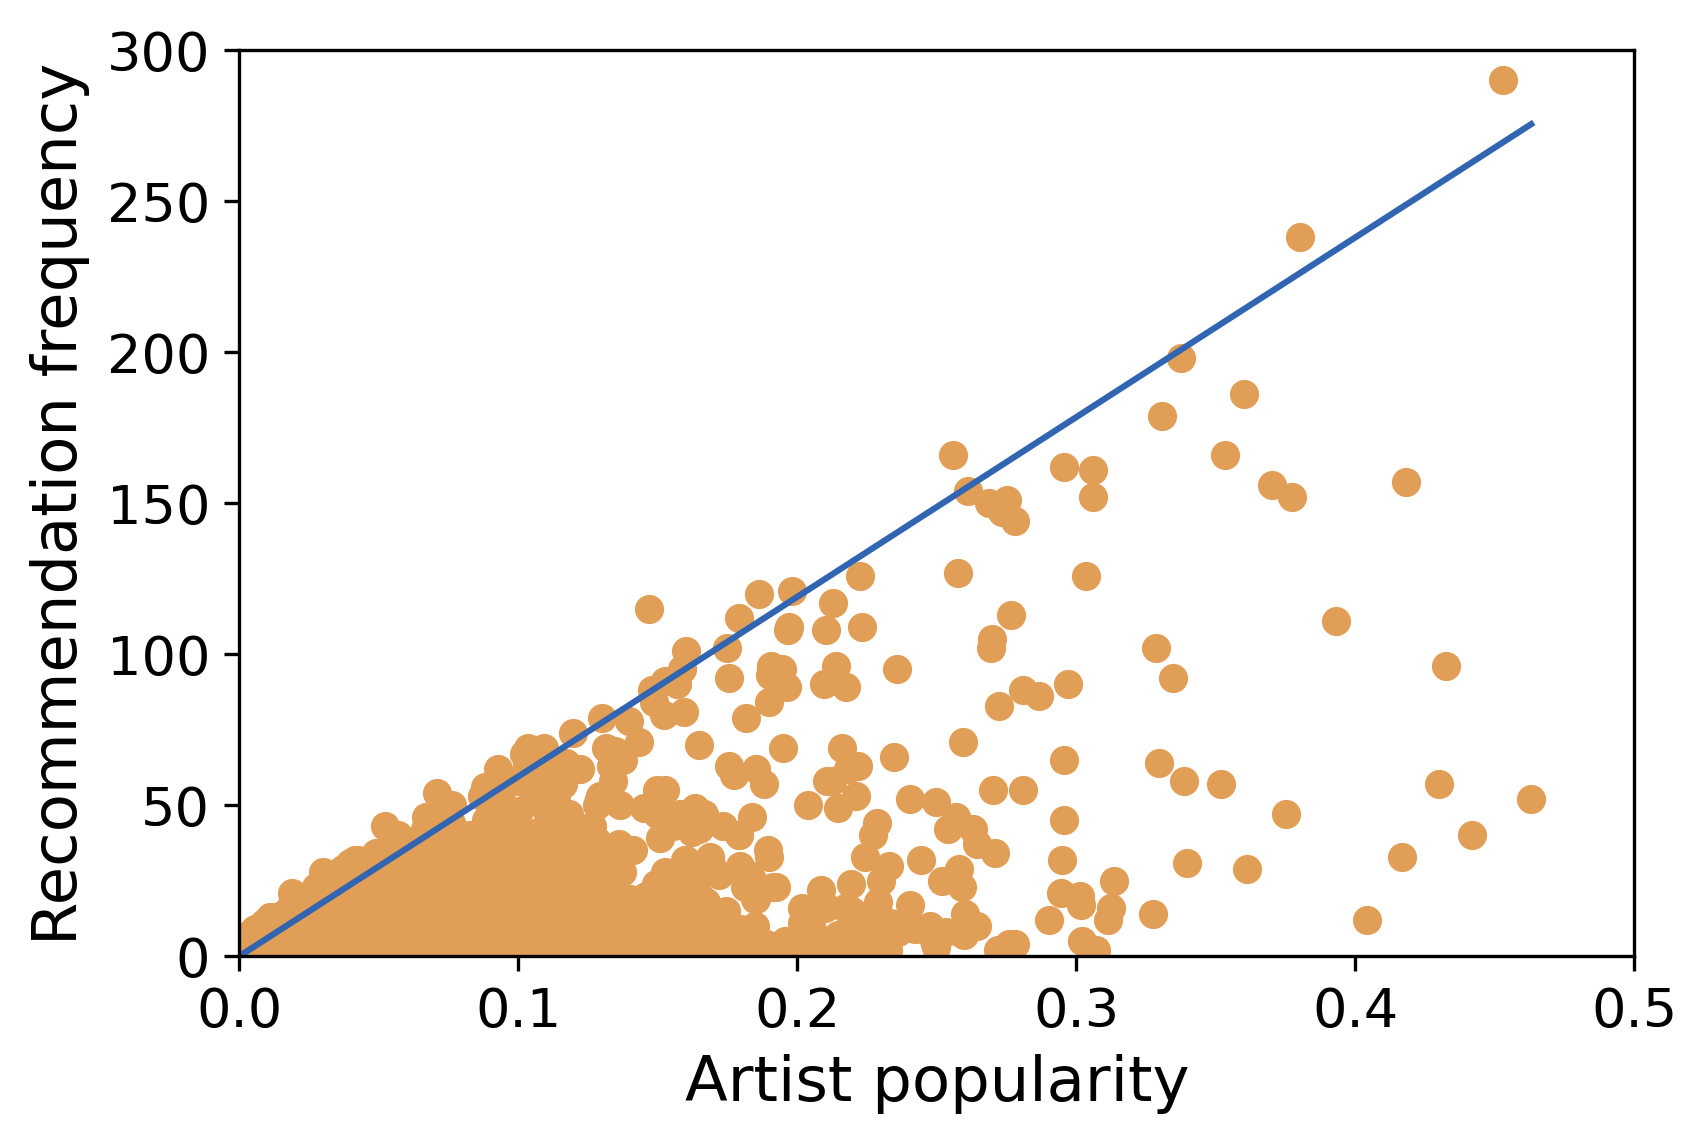
\includegraphics[width=35mm]{img/sampl_modif_2_UserKNNAvg.png} &   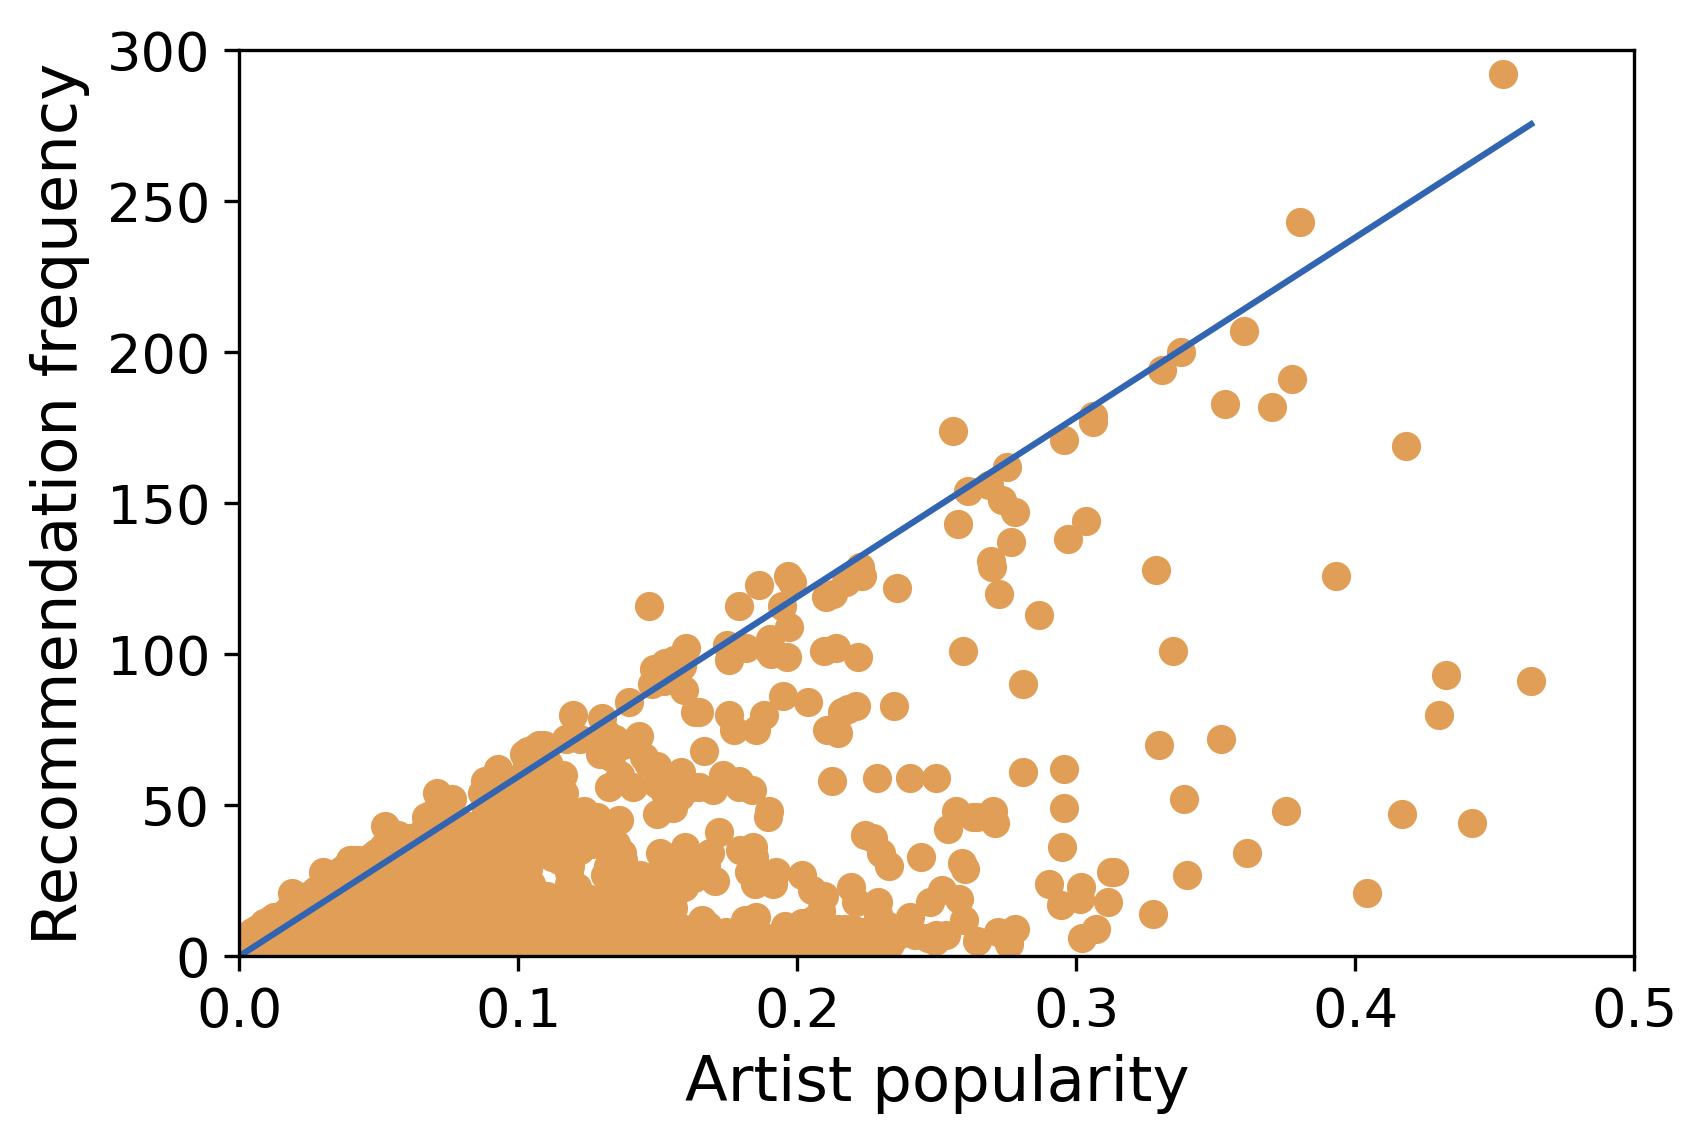
\includegraphics[width=35mm]{img/sampl_modif_2_UserKNN.png} \\
(a) UserKNNAvg & (b) UserKNN  \\[6pt]

  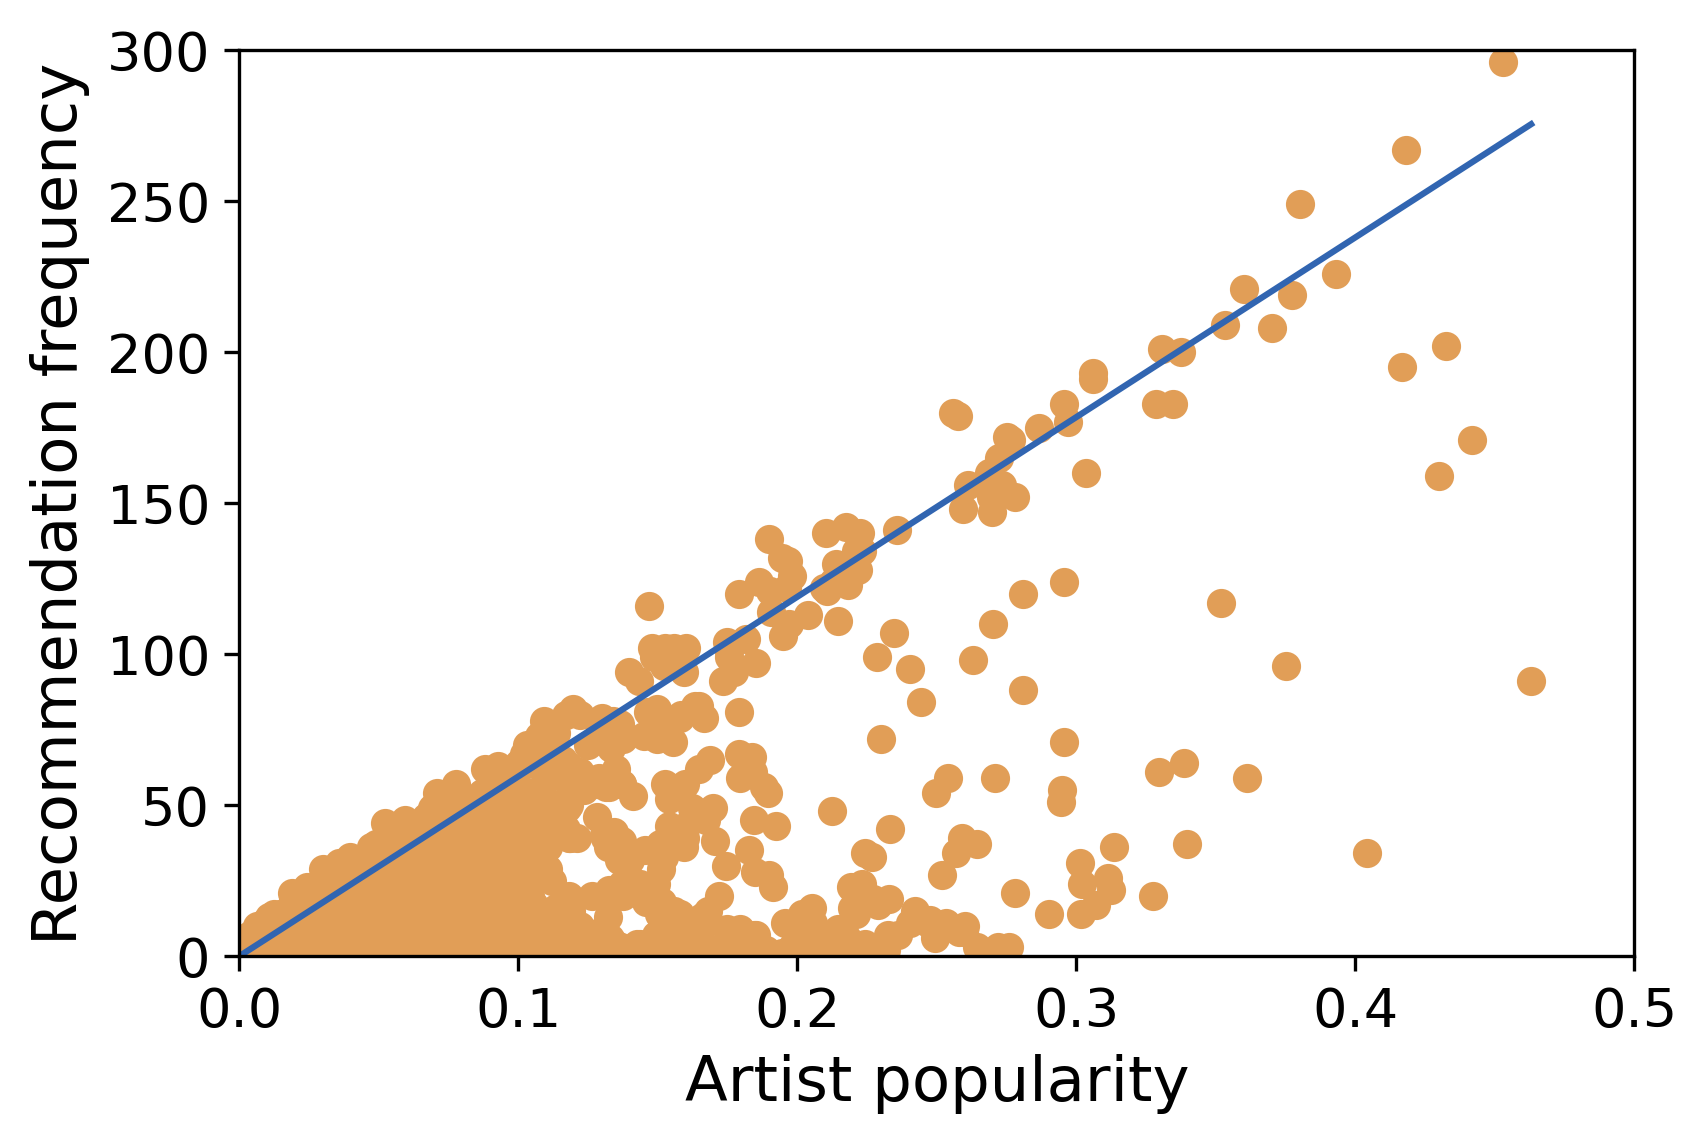
\includegraphics[width=35mm]{img/sampl_modif_2_UserItemAvg.png} &  
  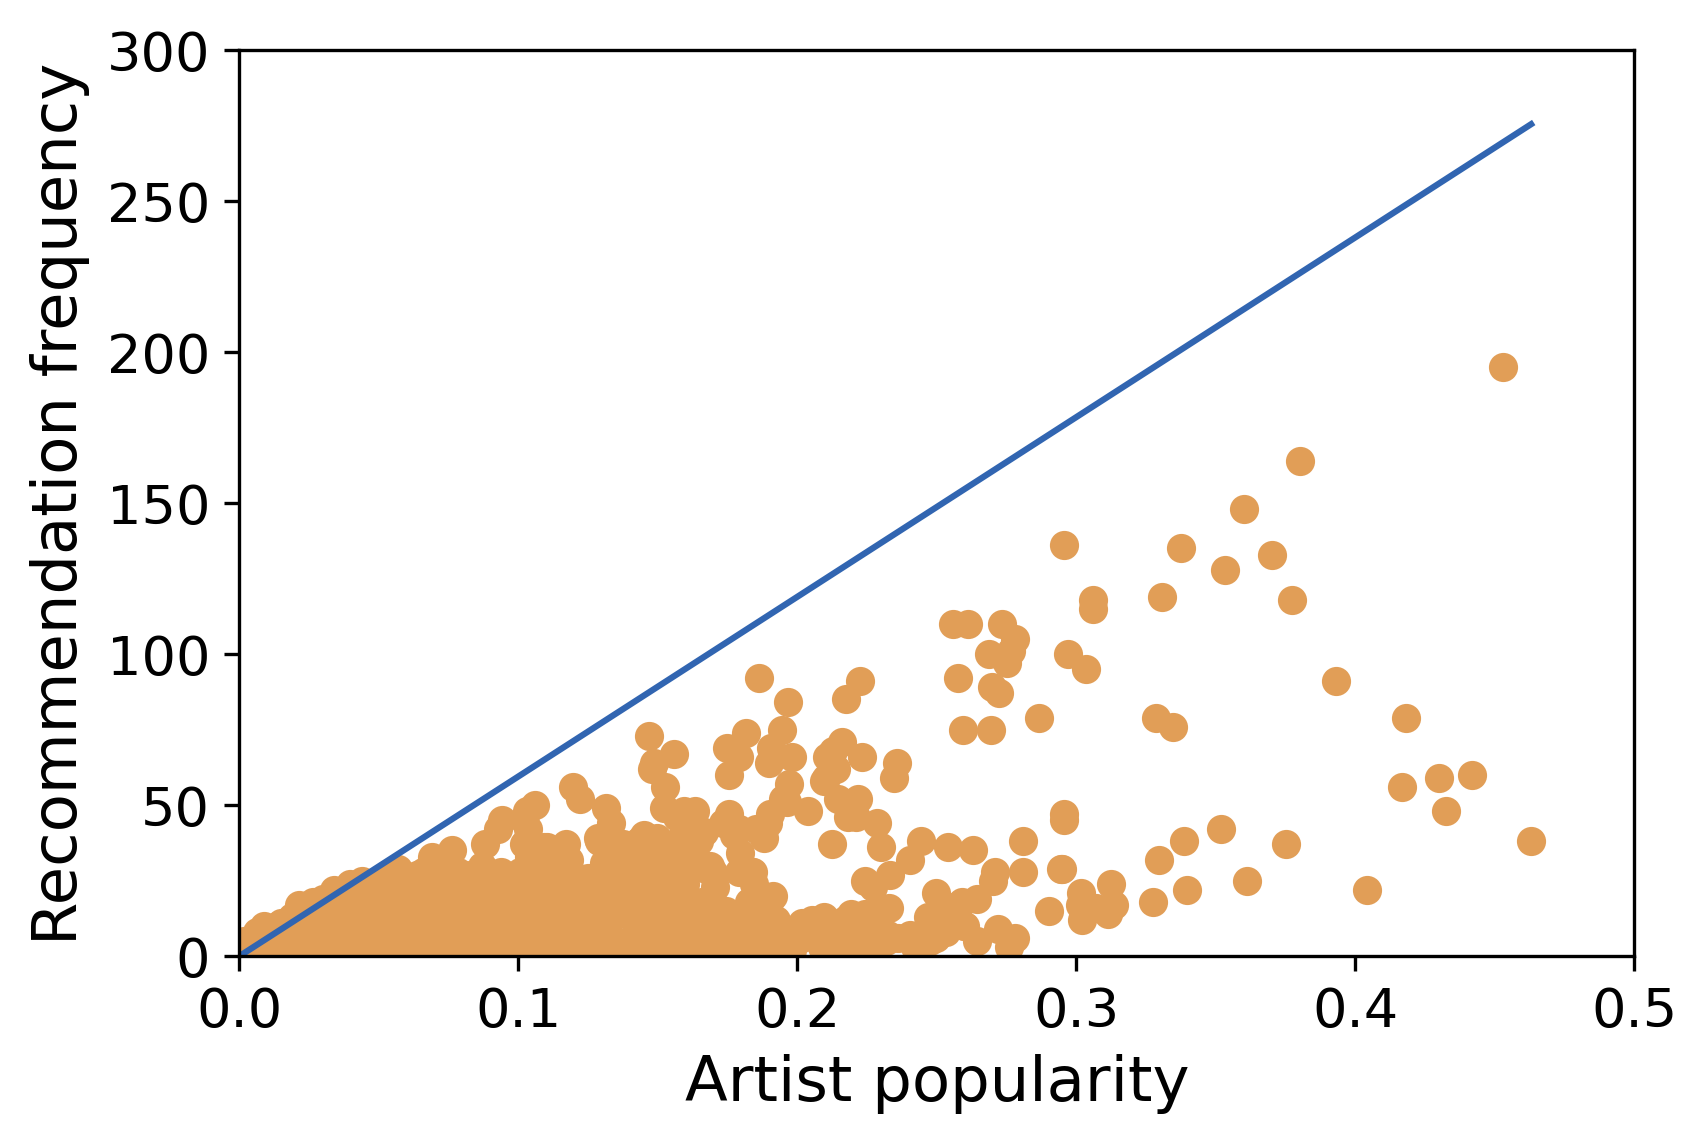
\includegraphics[width=35mm]{img/sampl_modif_2_NMF.png} \\
(c) UserItemAvg & (d) NMF \\[6pt]
\end{tabular}
\caption{Artist popularity against recommendation frequencies, using our modified prediction methodology.
A correlation between recommendation frequency and popularity is still observed, but the recommendation frequencies of highly popular artists
are spred below the blue line instead of very close to it.}
\label{fig:adap}
\end{figure}



The results regarding the fairness of our adapted 
predictions are now presented and compared to the standard
prediction methodology. When using our technique, 
for $n = 60$ and $m = 30$, the average resulting 
number of predictions is $\approx 28$. This happens because, 
sometimes the first top 60 artists extracted do not contain
$m_1$ artists from cluster 0 (low popularity),
reducing the average final number of predictions. 
This is a detail that can be improved in further
versions of our proposed algorithm, but which does
not necessarily cause any harm. As a consequence, 
we use $n = 28$ for the comparison with the standard 
top-$n$ method. 

Figures \ref{fig:std} and \ref{fig:adap} present the
artist popularities against its recommendation frequencies, 
with a straight line plotted for reference. 
For the standard prediction methodology, we observe a clear
positive correlation between frequency and popularity for all four
algorithms: popular items get the highest recommendation frequencies. 
In contrast, Figure \ref{fig:adap} shows a different pattern 
for the highest popularity items. Now they are not mostly 
close to the blue line, but rather wider spread below it. 
Correspondingly, as we have approximately the same total number
of recommendations being plotted in all figures,
this means that the less popular artists are now being more
frequently recommended as well. This result is more easily 
observable in the NMF model plot, where the gap between the straight
line and the low popularity values (<0.1) is reduced in 
Figure \ref{fig:adap}. 
 
 
We also present our findings in terms of the GAP(g)$_r$ \cite{pap_unfairness}, a metric of 
the average popularity of the artists recommended by
an algorithm $r$ to the users in group $g$, which in 
this work is represented by the mainstreaminess groups. In Figure \ref{fig:gap}, 
we examine how much the popularity of the predictions
differs from the expected popularity of the artists
in the user profiles of the test set, by plotting the
observed change in the GAP(g)$_r$ 
(namely $\Delta$ GAP(g)$_r$). 
For this metric, values close to 0 indicate fairness regarding
the popularity of the artists being predicted.


Figure \ref{fig:gap} shows the results for both the 
standard and our adapted prediction method. In 
agreement with what was observed in \cite{pap_unfairness},
the UserItemAvg algorithm has the highest values for all 
three groups. Regarding the comparison between the two
techniques, our adapted method seems to produce 
much fairer predictions. 
For all cases, the $\Delta$ GAP(g)$_r$ metric
is drastically reduced, especially for the NMF algorithm, 
for which the resulting predicted popularity is even
lower than the expected one. We think that this
happens because the NMF already had the lowest correlation
between popularity and recommendation frequency, so the
effect of our method was intensified in comparison to the
other three recommendation algorithms analysed here. 
This 
is a reason for us to believe that improvements can
still be made in our method, and that the estimated clustering
proportions should not be blindly accepted as the best option
for example. 

\begin{figure}[ht]
\centering
\begin{tabular}{cccc}
  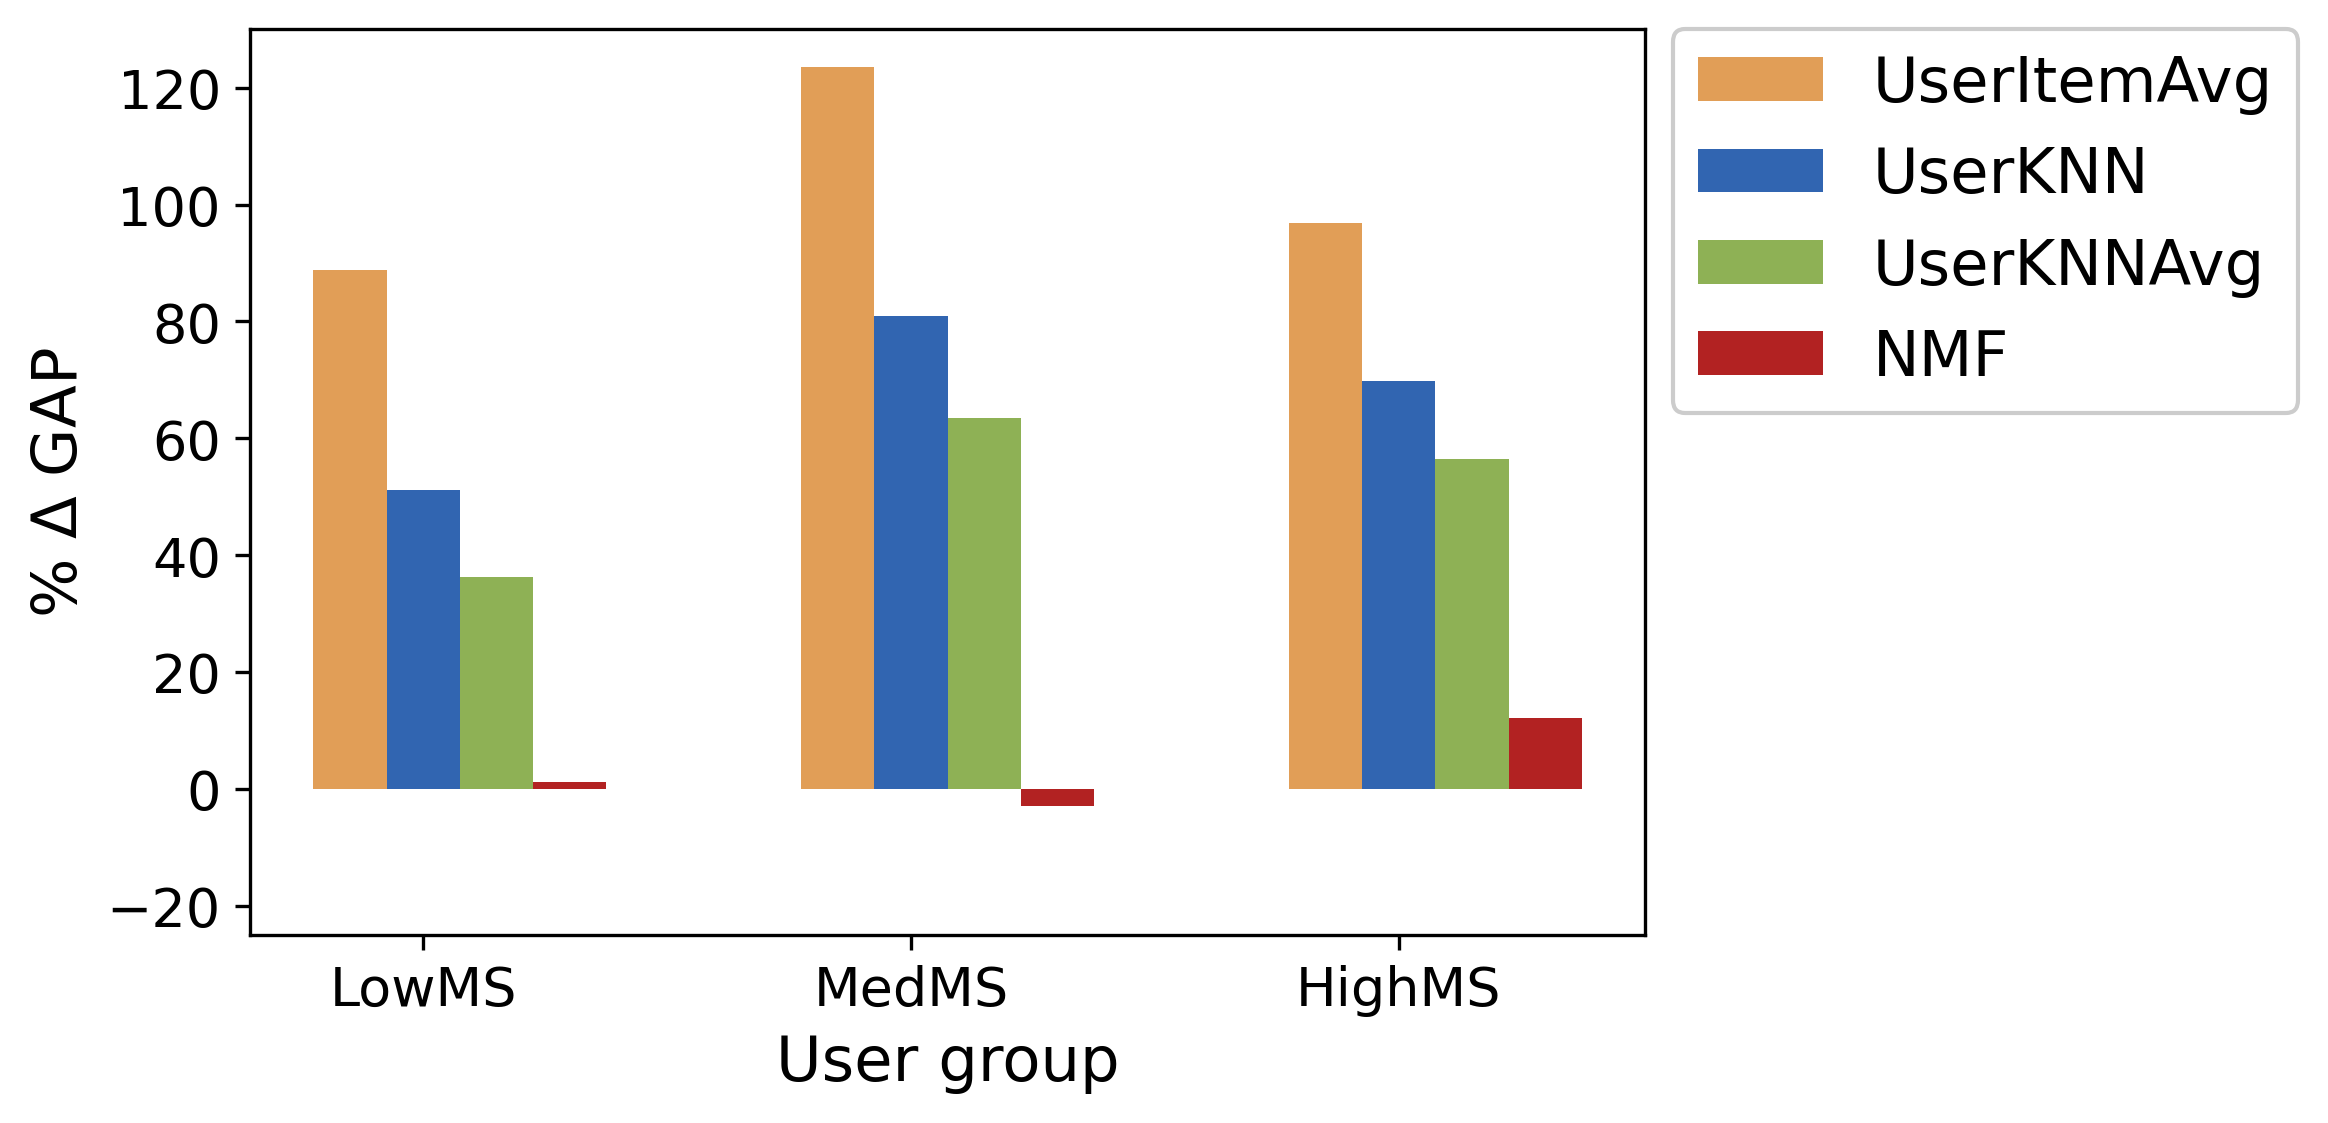
\includegraphics[width=75mm]{img/gap_analysis_28.png} \\
(a) Standard Prediction Method  \\[6pt]
  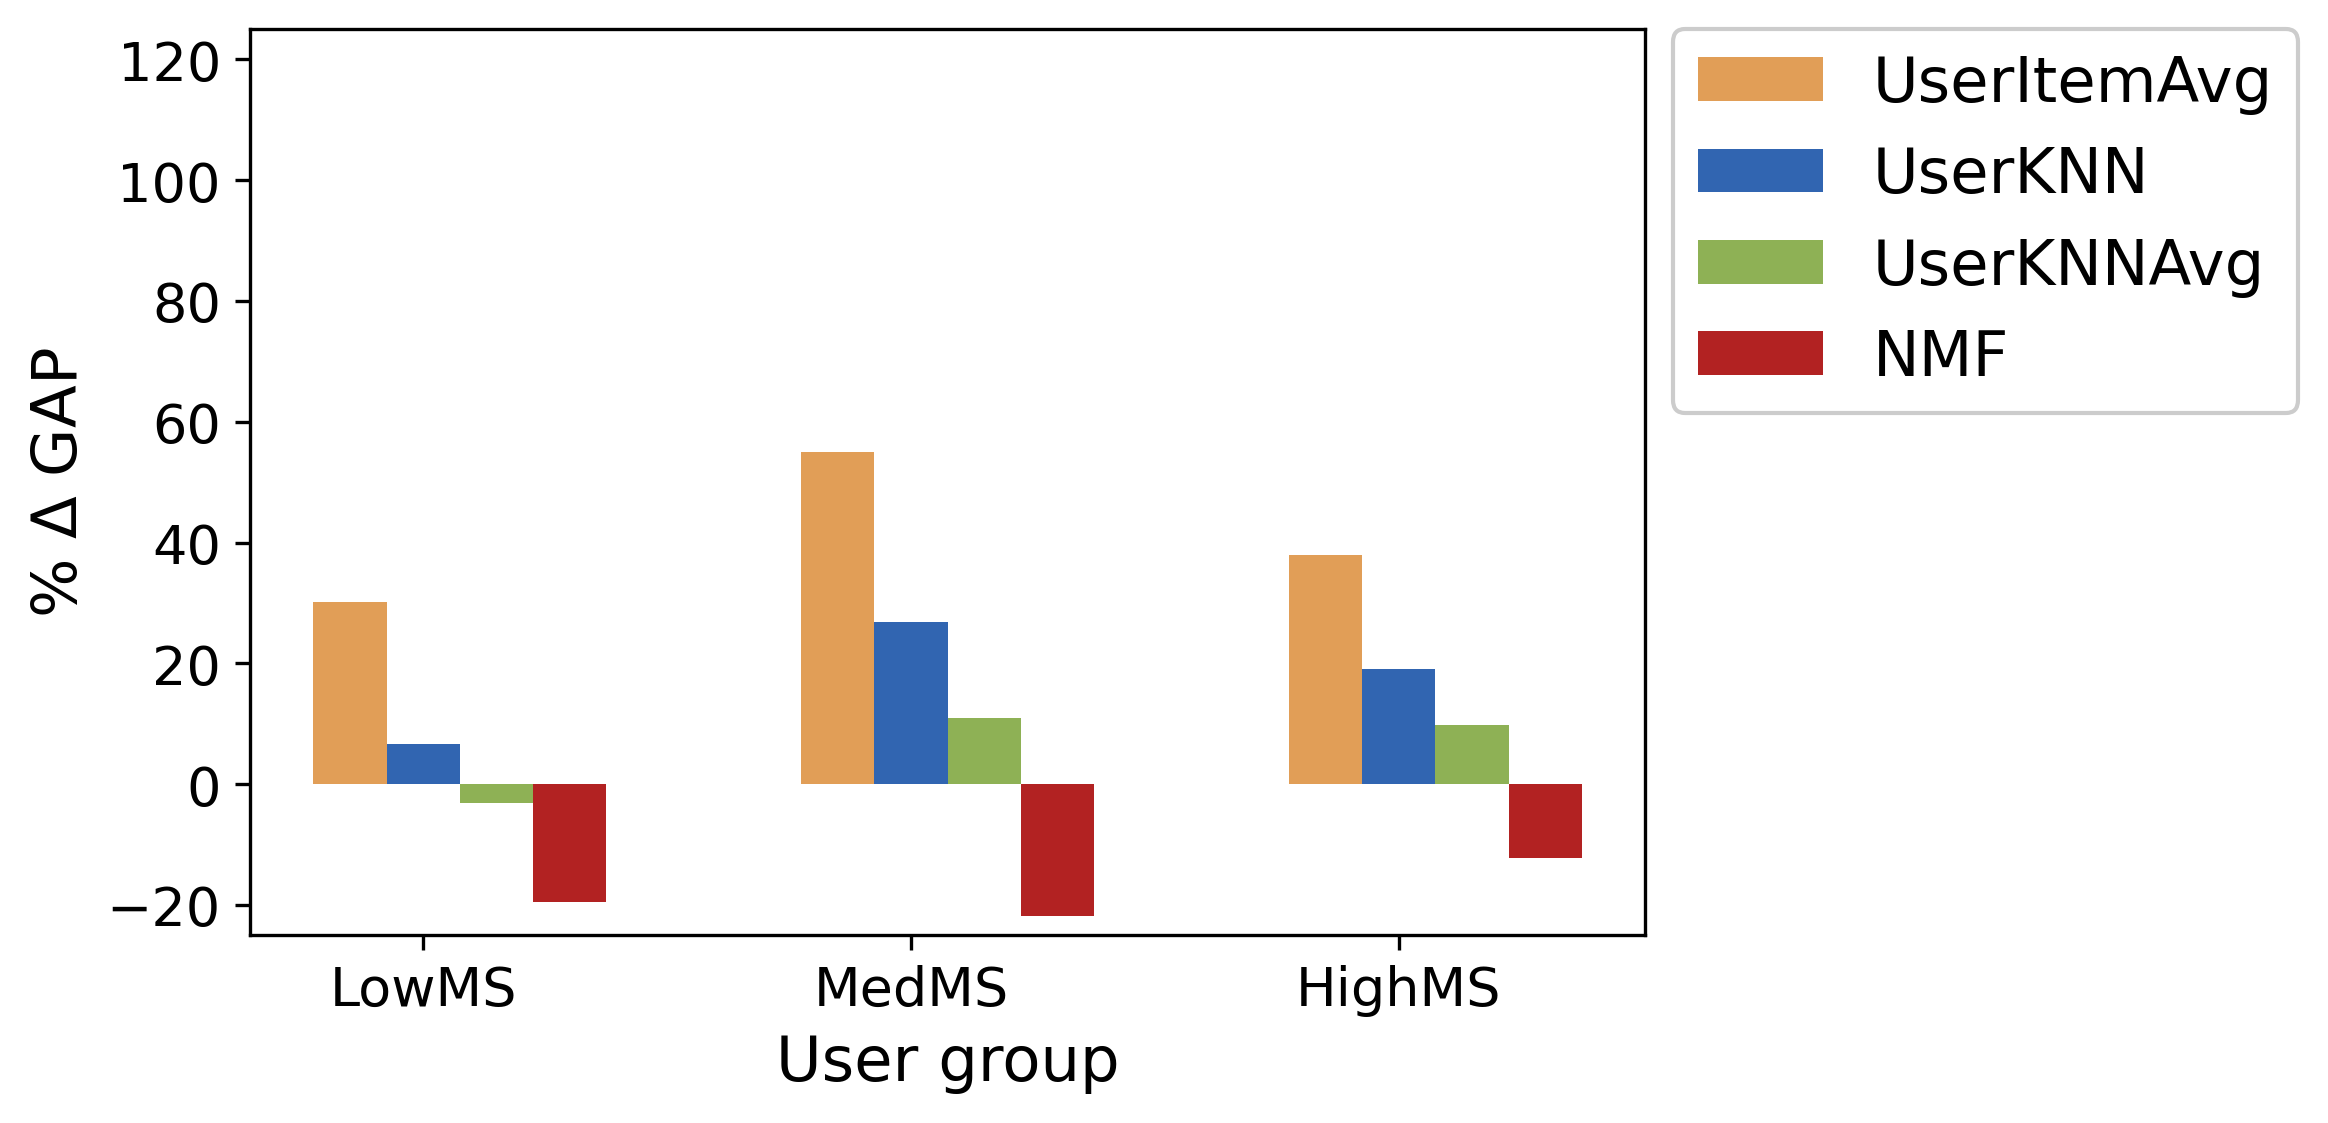
\includegraphics[width=75mm]{img/gap_analysis_modif_2.png} \\
(b) Adapted Predictions  \\[6pt]
\end{tabular}
\caption{Group Average Popularity change ($\Delta$ GAP)  
for  the three mainstreaminess groups (the lower the \%, the 
fairer the recommendations regarding popularity). 
The shapes of the distributions remain similar, but the  
$\Delta$ GAP (y-axis) values are drastically smaller 
after our adaption.}
\label{fig:gap}
\end{figure}

\subsection{Accuracy}\label{sec:pop_cluster}

The accuracy of recommender systems might be
evaluated via a few different
metrics, including the Mean Average Error (MAE),
which is more robust to outliers than the Mean Squared Error 
(MSE) \cite{willmott2005advantages}. In this section, we
assess the accuracy of the two prediction methods by calculating the MAE
for each user in the test set and subsequently taking the average 
of the results. The results are shown in Tables \ref{table:mae} and
\ref{table:mae_modif}. 

As seen in both tables, the accuracies vary between the algorithms, 
and the NMF produces the best results. Similarly, the Medium
mainstreaminess group (MedMS) has the lowest MAEs in all cases except 
for the UserKNN model. However, our biggest interest lies in
the differences between the two tables. Unexpectedly, our method
produces lower MAEs for all but the LowMS group in the NMF algorithm. We say that because improvements on the popularity
fairness do not necessarily imply accuracy improvements, 
so this is an additional advantage of our method. 





\begin{table}[ht]
\centering
\vspace{1.1}
\setlength\tabcolsep{1.5pt} 
\begin{tabular}{l | cccc}
  \hline
  \hline
  Group & UserItemAvg & UserKNN & UserKNNAvg & NMF \\ 
  \hline
  LowMS      & 73.25  &  87.79  & 84.11      & \textbf{55.6}  \\
  MedMS      & 72.86  &  91.83  & 81.52      & \textbf{51.98}  \\
  HighMS     & 80.86  &  90.37  & 85.97      & \textbf{65.23} \\
  \hline
  All        & 75.66  &  89.99  & 83.87      & \textbf{57.61} \\
   \hline
   \hline
\end{tabular}
\caption{Average MAE results for the state-of-the-art music  recommendation systems considered here, calculated using the Top 28 recommendations for each user. The best results are of the NMF model.}
\label{table:mae}
\end{table}


\begin{table}[ht]
\centering

\vspace{1.1}
\setlength\tabcolsep{1.5pt} 
\begin{tabular}{l | cccc}
  \hline
  \hline
  Group & UserItemAvg & UserKNN & UserKNNAvg & NMF \\ 
  \hline
  LowMS      & 66.46  &  79.35  & 76.55      & \textbf{55.73}  \\
  MedMS      & 61.88  &  77.84  & 70.21      & \textbf{47.34}  \\
  HighMS     & 68.52  &  74.99  & 73.19      & \textbf{56.53} \\
  \hline
  All        & 65.62  &  77.39  & 73.32      & \textbf{53.20} \\
   \hline
   \hline
\end{tabular}
\caption{Average MAE results for the state-of-the-art music  recommendation systems considered here, calculated using the
predictions made by our method. The best results are of the NMF model.}
\label{table:mae_modif}
\end{table}


The differences between the results of the two methods
are more explicitly presented in Table \ref{tab:mae_delta}, 
where we show the percentual  differences  between  the 
average MAE  for  the  standard  method  and  our  adapted  method, given by $(-(MAE(g)_{std} - MAE(g)_{adp})/MAE(g)_{std}$. This metric will give 
us a percentage notion of the improvement of our 
method in relation to the standard technique. As seen 
in the results, the model that has the highest improvements 
is the UserKNN, followed by the UserItemAvg, UserKNNAvg 
and then the NMF, and the user group with the highest improvement is the HighMS.



\begin{table}[ht]
\centering
\vspace{1.1}
\setlength\tabcolsep{1.5pt} 
\begin{tabular}{l | cccc}
  \hline
  \hline
  Group & UserItemAvg & UserKNN & UserKNNAvg & NMF \\ 
  \hline
  LowMS      & -9.27   & -9.61    & -8.99       & 0.23 \\
  MedMS      & -15.07  & -15.23   & -13.87      & -8.93 \\
  HighMS     & \textbf{-15.26}  & \textbf{-17.02}   & \textbf{-14.87}      & \textbf{-13.34} \\
  \hline
  All        & -13.27  & -14.00   & -12.58      & -7.65 \\
   \hline
   \hline
\end{tabular}
\caption{Percentual differences between the average MAE for the standard method and our adapted method $(-(MAE(g)_{std} - MAE(g)_{adp})/MAE(g)_{std}$. We observe mostly
positive values, implying an overall decrease in the MAE. The highest improvements happen for the HighMS group.}
\label{tab:mae_delta}
\end{table}



\section{Conclusions}\label{sec:discussion}

Equal opportunity and fairness are emerging themes in 
many areas of machine learning, including recommender
systems. As one of its main users, MIR researchers have
been increasingly turning their attention to these 
topics. The importance of said research makes itself 
clear when we consider how much artificial intelligence
currently affects our society. As a consequence, 
investigating and coming up with ways of reducing biases 
in our analysis has become more important than ever.

In this paper, we have proposed a novel method to 
make predictions for music recommender systems, aiming to reduce the popularity bias inherent in the current algorithms. Our 
main concern is to improve fairness from the
perspective of the users, by recommending them artists
that are actually in consonance with their preferences, 
and from the perspective of the artists, by not 
giving unwarranted preference to highly popular 
items. 

As observed in the experiments, we have achieved both goals. Our method leads to highly popular artists being recommended less
than with the standard approach, and the recommendations better
approximate the expected popularity of the artists in
each user profile. In addition, the Mean Average Error
metric has also improved, showing that the accuracy of 
our predictions is positively affected. Those results
were observed for the three different user groups
(low, medium and high mainstreaminess), with the 
highest improvements associated with the high mainstreaminess
group, telling us that, previously, the algorithms
were affecting this group with biased predictions the most.

Our proposed method is not perfect and there is still 
room for research on the topic. Though we have not
observed drawbacks yet, in future work we
intend to explore ways to extend the method, 
as well as make more experiments using a bigger pool of 
recommendation algorithms. It would also be interesting
to compare the method to other fairness-focused 
approaches, such as \cite{wang2016multi}.
Moreover, the bias 
context can also be modified, and the same technique
might be utilized to improve fairness regarding 
other aspects of music recommendation 
(age, geography, genre preference, etc).  



% talk more of the three groups 

% For bibtex users:
\bibliography{ISMIRtemplate}

% For non bibtex users:
%\begin{thebibliography}{citations}
%
%\bibitem {Author:00}
%E. Author.
%``The Title of the Conference Paper,''
%{\it Proceedings of the International Symposium
%on Music Information Retrieval}, pp.~000--111, 2000.
%
%\bibitem{Someone:10}
%A. Someone, B. Someone, and C. Someone.
%``The Title of the Journal Paper,''
%{\it Journal of New Music Research},
%Vol.~A, No.~B, pp.~111--222, 2010.
%
%\bibitem{Someone:04} X. Someone and Y. Someone. {\it Title of the Book},
%    Editorial Acme, Porto, 2012.
%
%\end{thebibliography}

\end{document}

